\documentclass[a4paper]{article}
\usepackage{fancyhdr}
\usepackage[usenames, dvipsnames]{xcolor}
\usepackage{graphicx,hyperref,amsmath}
\usepackage[top=3cm,bottom=3cm,left=3cm,right=3cm]{geometry}
\hypersetup{
	colorlinks,
	citecolor=black,
	filecolor=black,
	linkcolor=black,
	urlcolor=black
}
\newcommand{\HRule}{\rule{\linewidth}{0.5mm}}
\pagestyle{fancy}
\lfoot{\small \color{gray}Tom Peerdeman - 10266186}
\cfoot{\thepage}
\rfoot{\small \color{gray}Ren\'e Aparicio Sa\'ez - 10214054}
\lhead{\small \color{gray}Echofilter}
\begin{document}
	\begin{titlepage}
	\begin{center}
		\textsc{\Large Multimedia}\\[0.5cm]
		\HRule \\[0,4cm]
		\textsc{\huge \bfseries Echofilter}
		\HRule \\[8cm]
		\begin{minipage}{0.4\textwidth}
			\begin{flushleft}\large
				\emph{Auteurs: Tom Peerdeman \& Ren\'e Aparicio Saez}\\
			\end{flushleft}
		\end{minipage}
		\begin{minipage}{0.4\textwidth}
			\begin{flushright}\large
			\emph{Datum: 18-06-2012\\\'}\\
			\end{flushright}
		\end{minipage}
	\end{center}
	\end{titlepage}

	\tableofcontents
	\newpage

	\section{Inleiding}\label{sec:inleiding}
		Een echo treedt op als geluid weerkaatst op een opppervlak, waarna deze wordt teruggekaatst naar de originele bron van het geluid. De tijd die hier tussen zit hangt af van de afstand van de bron tot aan het weerkaatsende oppervlak. Door welk materiaal het geluid zich moet voortplanten is ook een belangrijke factor.\\
Op een computer kan dit proces worden nagebootst. Hiertoe moet een echofilter worden gebouwd, die een echo reproduceert op een aangegeven interval.
\\[1.5cm]
	\begin{figure}[h]
		\begin{center}
			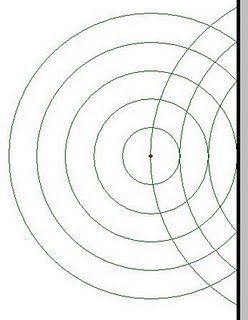
\includegraphics[width=0.5\textwidth]{echo.jpg}
			\caption{Schematische weergave van een echo}
		\end{center}
	\end{figure}
\newpage

	\section{Opbouw}
	\subsection{Geluid}
		Om een echo te maken is eerst geluid nodig. Hier kan een willekeurig gekozen geluidsbestand voor genomen worden. Processing levert een aantal voorbeeld geluidsbestanden mee in zijn voorbeelden, deze zijn een prima uitgangspunt om mee te beginnen.
	\subsection{Circular Buffer}
		Een echo is feitelijk het geluid wat op een bepaald moment hoorbaar is met hierbij opgeteld teruggekaatst geluid dat hoorbaar is. In het programma moet geluid dat al door de bron is uitgezonden worden onthouden om na een bepaald interval weer hoorbaar te zijn. Hiervoor worden circular buffers gebruikt. Het geluid wordt per sample opgeslagen in deze buffer. Echter is het onmogelijk om van te voren te weten hoeveel ruimte er in de buffer nodig is. Het is dus handig om de buffer groter te kunnen maken als deze vol zit. Op het moment dat de buffer vol zit wordt deze twee keer zo groot gemaakt. Zo wordt er voorkomen dat de buffer weer snel volraakt.
	\subsection{Echo effect}
		Een geluid op een computer bestaat uit twee kanalen, links en rechts. De echo moet dus per kanaal worden toegevoegd. Er zijn dus twee circular buffers nodig, \'e\'en per kanaal. In de circular buffer zit het originele geluid opgeslagen. Aan dit originele geluid moet een echo worden toegevoegd. Deze echo wordt bepaald door een aangegeven tijdsinterval en hoe hard deze echo is. Deze waardes kunnen statisch of dynamisch zijn. Het tijdsinterval zorgt ervoor dat uit de circular buffer waardes worden genomen die in het verleden zijn afgespeeld. Deze waarde vermenigvuldigd met een aangegeven volume bepalen de waarde van de echo. Deze waarde wordt opgeteld bij het originele geluid, waarna het wordt afgespeeld.
	\subsection{Dynamische variabelen}
		Het is als gebruiker uiteraard veel fijner om zelf invloed op een programma te hebben terwijl deze loopt. Bij het echo filter zijn daarom twee dynamisch aan te passen variabelen gemaakt, het tijdsinterval van de decho en het volume hiervan. Dit is gedaan door middel van twee schuifbalken. Processing geeft een voorbeeld programma mee onder de naam 'Scrollbar' in de categorie 'GUI' in de categorie 'Topics'. Twee van deze scrollbars zijn gebruikt voor de variabelen. Het tijdsinterval loopt van 0 tot en met 9.9. Het volume loopt van 0 tot en met 0.99. Het volume van het live geluid en het echo geluid is samen 1 (100\%).

\newpage

	\section{Experimenten}
	\subsection{Standaard echo}
		De scrollbars staan standaard in het midden. Dit levert een tijdsinterval van 5 seconden op en een volume van 0.5 (50\%). De eerste vijf seconden speelt het geluid zich normaal af, vervolgens is er duidelijk een echo hoorbaar.
	\begin{figure}[h]
		\begin{center}
			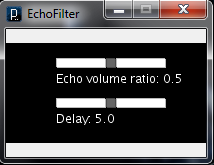
\includegraphics[width=0.5\textwidth]{echofilter.png}
			\caption{Standaard programma uiterlijk}
		\end{center}
	\end{figure}
	\subsection{Beste echo}
		Om de beste echo te produceren is een tijdsinterval van 0.3 seconden nodig en een volume van 0.2 (20\%). Er is dan heel duidelijk een herhaling van het voorgaande geluid te horen.

\newpage

	\section{Conclusie}
		Het echofilter produceerd een goed realistisch klinkende echo. Het tijdsinterval en volume van de echo kunnen op een goede makkelijke manier handmatig worden aangepast. Hiermee kan een denkbeeldig afstand tussen bron en weerkaatsend oppervlak gerealiseerd worden. Het programma bevat echter \'e\'en vervelende fout. Zodra handmatig een nieuw tijdsinterval wordt aangegeven worden de circular buffers geleegd. De nieuwe echo is niet direct hoorbaar, maar pas nadat \'e\'en maal de aangegeven tijdsinterval is verstreken. Vervolgens doet de echo het wel weer goed. 
		
\newpage

	\section{Code}
	\subsection{EchoFilter.pde}
\begin{verbatim}
/*
 * File: EchoFilter.pde
 *
 * This file contains the setup method wich starts the audioplayer with the 
 * echo effect enabled.
 *
 * Author: René Aparicio Saez
 * Student nr.: 10214054
 *
 * Author: Tom Peerdeman
 * Student nr.: 10266186
 *
 * Date: 16/06/2012
 *
 */

import ddf.minim.*;
import ddf.minim.effects.*;
import processing.opengl.*;

private Minim minim;
private AudioPlayer player;
private EchoEffect effect;
private ScrollBar delayBar;
private ScrollBar volumeBar;
private float delayPos;
private float volumePos;

public void setup(){
    size(200, 100, OPENGL);
    volumeBar = new ScrollBar(50, 20, 110, 10, 5);
    delayBar = new ScrollBar(50, 60, 110, 10, 5);
    
    minim = new Minim(this);
    player = minim.loadFile("groove.mp3", 1024);
    effect = new EchoEffect();
    player.addEffect(effect);
    player.loop();
}

public void draw(){
    background(0);
    // Set text color
    fill(0xFF, 0xFF, 0xFF);
    text("Echo volume ratio: " + floor((volumeBar.getPos() - 50)) / 100f, 50,
        40);
    text("Delay: " + floor((delayBar.getPos() - 50)) / 10f, 50, 80);
    
    volumeBar.update();
    delayBar.update();
    volumeBar.display();
    delayBar.display();
    
    // Only update the effect if the value of one of the bars has changed.
    if(volumePos != volumeBar.getPos()){
        volumePos = volumeBar.getPos();
        effect.setEchoVolume(floor((volumePos - 50)) / 100f);
    }
    if(delayPos != delayBar.getPos()){
        delayPos = delayBar.getPos();
        effect.setDelay(floor((delayPos - 50)) / 10f);
    }
}

public void stop(){
    player.close();
    minim.stop();
    super.stop();
}
\end{verbatim}
\newpage
\subsection{CircularBuffer.pde}
\begin{verbatim}
/*
 * File: CircularBuffer.pde
 *
 * This file contains an implementation of a float circular buffer.
 * The buffer is dynamic: when the buffer is full it will enlarge itself.
 *
 * Author: René Aparicio Saez
 * Student nr.: 10214054
 *
 * Author: Tom Peerdeman
 * Student nr.: 10266186
 *
 * Date: 16/06/2012
 *
 */

class CircularBuffer{
    private float[] buffer;
    private float[] bufferResize;
    private int head;
    private int tail;
    public int fill;
    
    public CircularBuffer(int initCap){
        head = 0;
        tail = 0;
        fill = 0;
        buffer = new float[initCap];
    }
    
    public void addSample(float v){
        // Buffer full, resize
        if(fill == buffer.length){
            bufferResize = new float[buffer.length * 2];
            if(head == 0){
                arraycopy(buffer, 0, bufferResize, 0, buffer.length);             
            }else{
                arraycopy(buffer, tail, bufferResize, 0, buffer.length - tail);
                arraycopy(buffer, 0, bufferResize, buffer.length - tail, head);
            }
            head = buffer.length;
            tail = 0;
            buffer = bufferResize;
            bufferResize = null;
        }
        
        buffer[head++] = v;
        fill++;
        head %= buffer.length;
    }
    
    public float getSample(){
        if(fill == 0){
            return 0f;
        } 

        float get = buffer[tail++];
        tail %= buffer.length;
        fill--;
        return get;
    }
    
    public void clear(){
        tail = 0;
        head = 0; 
        fill = 0;
    }
}
\end{verbatim}
\newpage
	\subsection{EchoEffect.pde}
	\begin{verbatim}
/*
 * File: EchoEffect.pde
 *
 * This file contains an implementation of an echo effect.
 * The echo effect uses two circular buffers, one for each channel.
 * In this buffer are already played samples stored.
 * When a new sample is processed the sample 'delayLength' samples
 * before this sample is combined with the to processed sample.
 *
 * Author: René Aparicio Saez
 * Student nr.: 10214054
 *
 * Author: Tom Peerdeman
 * Student nr.: 10266186
 *
 * Date: 16/06/2012
 *
 */

public class EchoEffect implements AudioEffect{
    private CircularBuffer bufLeft;
    private CircularBuffer bufRight;
    private int delayLength;
    private float echoVolume;
    private float nonEchoVolume;
    
    public EchoEffect(){
        // Initialize volume & delay
        setDelay(0.2f);
        setEchoVolume(0.3f);

        // Initialize buffers
        bufLeft =    new CircularBuffer(delayLength + 1);
        bufRight =    new CircularBuffer(delayLength + 1);
    }
    
    public void setDelay(float delay){
        delayLength = (int) (44100 * delay);
        if(bufLeft != null){
            // Clear required otherwise older data than we want is mixed in.
            bufLeft.clear();
            bufRight.clear();
        }
    }
    
    public void setEchoVolume(float vol){
        echoVolume = vol;
        nonEchoVolume = 1f - vol;
    }
    
    public void process(float[] samp){
        for(int i = 0; i < samp.length; i++){
            bufLeft.addSample(samp[i]);
            if(bufLeft.fill >= delayLength){
                // Buffer full enough, mix it
                samp[i] = samp[i] * nonEchoVolume;
                samp[i] += bufLeft.getSample() * echoVolume;
            }
        }
    }

    public void process(float[] left, float[] right){
        for(int i = 0; i < left.length; i++){
            bufLeft.addSample(left[i]);
            bufRight.addSample(right[i]);
            
            // Buffer full enough, mix it
            if(bufLeft.fill >= delayLength){
                left[i] = left[i] * nonEchoVolume;
                left[i] += bufLeft.getSample() * echoVolume;
                right[i] = right[i] * nonEchoVolume;
                right[i] += bufRight.getSample() * echoVolume;
            }
        }
    }
}
	\end{verbatim}
\newpage
	\subsection{Scrollbar}
	\begin{verbatim}
/*
 * File: ScrollBar.pde
 *
 * Source: Processing Examples. Example 'Scrollbar' in category GUI in category Topics
 * Look up date: 14/06/2012
 *
 * Author: René Aparicio Saez
 * Student nr.: 10214054
 *
 * Author: Tom Peerdeman
 * Student nr.: 10266186
 *
 * Date: 16/06/2012
 *
 */

public class ScrollBar{
    private int swidth, sheight;        // width and height of bar
    private int xpos, ypos;                // x and y position of bar
    private float spos, newspos;        // x position of slider
    private int sposMin, sposMax;        // max and min values of slider
    private int loose;                    // how loose/heavy
    private boolean over;                // is the mouse over the slider?
    private boolean locked;

    public ScrollBar(int xp, int yp, int sw, int sh, int l){
        swidth = sw;
        sheight = sh;
        int widthtoheight = sw - sh;
        xpos = xp;
        ypos = yp-sheight/2;
        spos = xpos + swidth/2 - sheight/2;
        newspos = spos;
        sposMin = xpos;
        sposMax = xpos + swidth - sheight;
        loose = l;
    }

    public void update(){
        if(over()){
            over = true;
        }else{
            over = false;
        }
        if(mousePressed && over){
            locked = true;
        }
        if(!mousePressed){
            locked = false;
        }
        if(locked){
            newspos = constrain(mouseX-sheight/2, sposMin, sposMax);
        }
        if(abs(newspos - spos) > 1){
            spos = spos + (newspos-spos)/loose;
        }
    }

    private int constrain(int val, int minv, int maxv){
        return min(max(val, minv), maxv);
    }

    private boolean over() {
        if(mouseX > xpos && mouseX < xpos+swidth
            && mouseY > ypos && mouseY < ypos+sheight){
            return true;
        }else{
            return false;
        }
    }

    public void display(){
        fill(255);
        rect(xpos, ypos, swidth, sheight);
        if(over || locked){
            fill(153, 102, 0);
        }else{
            fill(102, 102, 102);
        }
        rect(spos, ypos, sheight, sheight);
    }

    public float getPos(){
        return spos;
    }
}
	\end{verbatim}


\end{document}
